\subsection{Overall Framework}
\label{sec:overall}

\rev{SynGS is developed as a sparse-view 3D Gaussian Splatting}~\cite{Kerbl23_3DGS} \rev{framework that combines explicit geometric initialization, depth-guided point cloud densification, and visibility-aware optimization.} Figure~\ref{fig:framework} \rev{illustrates the overall pipeline, which takes sparsely captured images and their corresponding foreground masks as input.} While recent variants organize Gaussians with structured scaffolds~\cite{Lu24_ScaffoldGS}, SynGS focuses on silhouette-based initialization and depth-guided densification under sparse posed inputs.

\begin{figure}[ht]
\centering
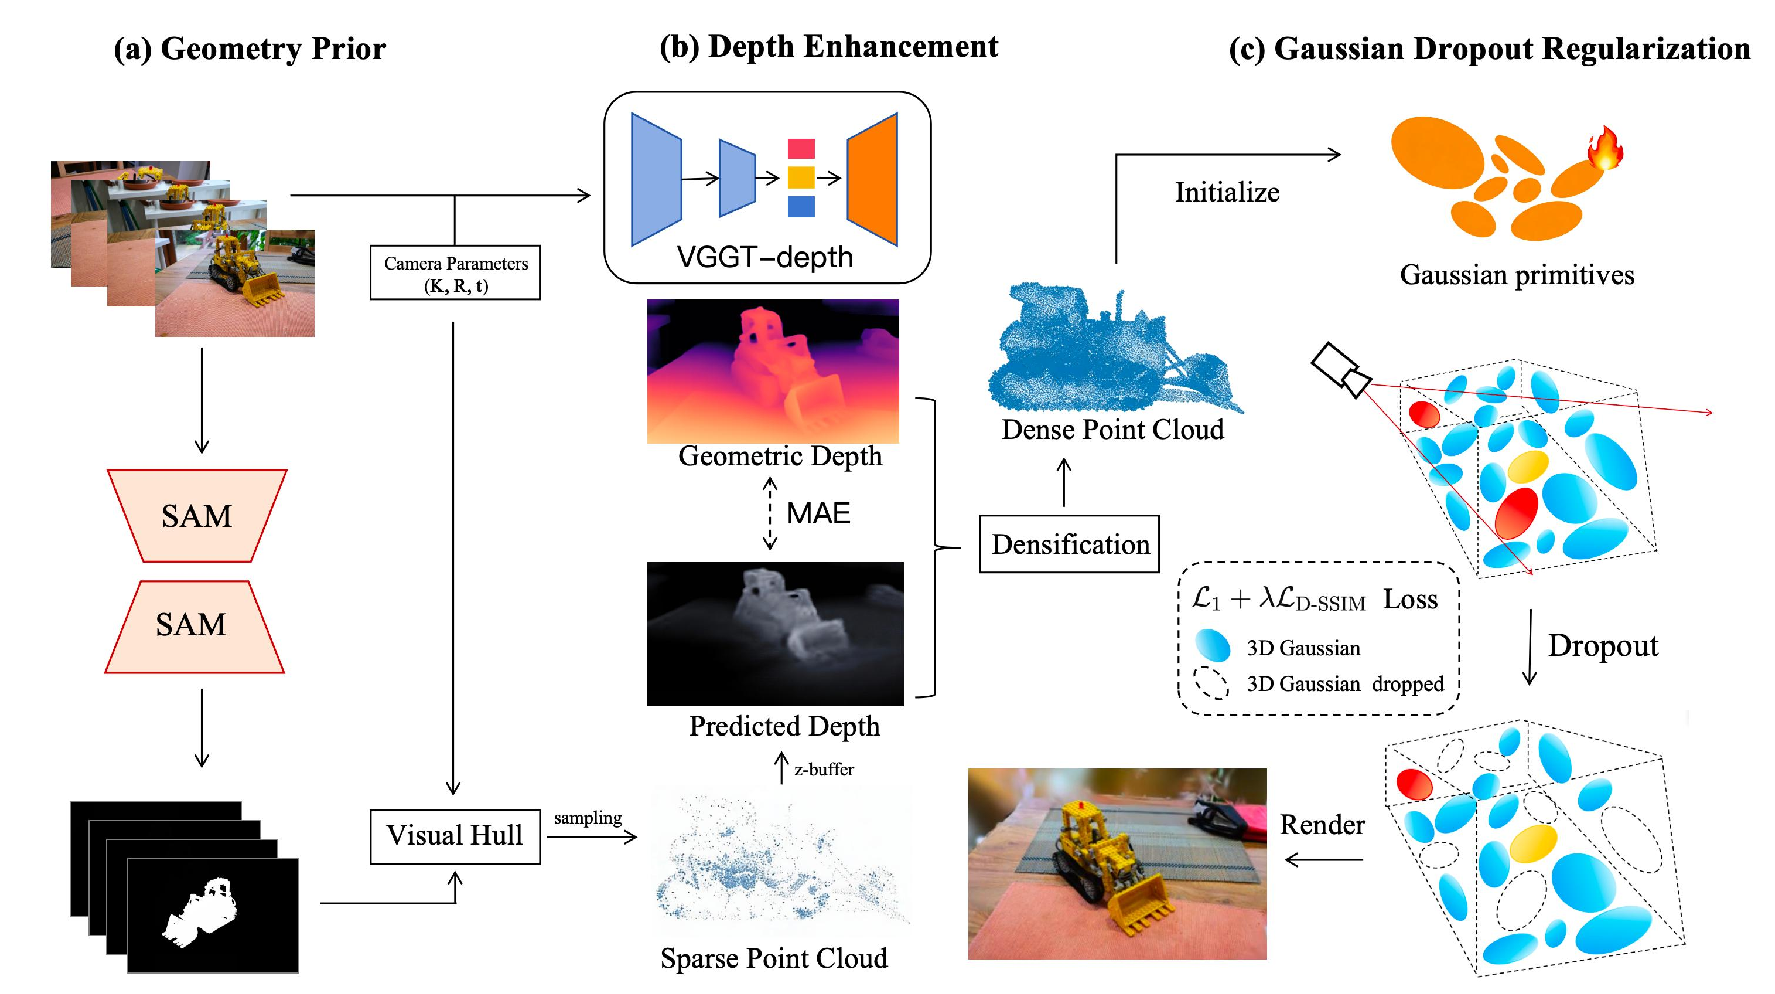
\includegraphics[width=0.90\textwidth]{figures/framework.pdf}
\caption{\label{fig:framework} Overview of the SynGS pipeline. The third stage applies Dynamic Visibility Regularization (DVR).}
\end{figure}

First, \textbf{Visual Hull Initialization} constructs a coarse geometric prior from multi-view silhouettes and generates an initial point cloud. Then, \textbf{VGGT-Guided Densification} exploits cross-view depth priors to supplement missing geometry and produce a depth-enhanced point cloud for Gaussian initialization. Finally, \textbf{Dynamic Visibility Regularization (DVR)} is applied during 3DGS optimization to rebalance supervision under sparse visibility and reduce overfitting. The complete process proceeds from the Visual Hull point cloud, through depth densification and Gaussian initialization, to DVR-regularized optimization.
